% MASTER'S LEVEL AI PRESENTATION - WEEK 1 (STRICT RECONSTRUCTION)
% Course: AI for Year One Business Administration
% Lecturer: Awara Bakhtiyar Rasool
% University: Salahaddin University-Erbil
% ============================================================================

\documentclass[aspectratio=169,10pt]{beamer}

% THEME & PACKAGES
\usetheme{metropolis}
\usepackage{graphicx}
\usepackage{tikz}
\usetikzlibrary{positioning,shapes,arrows,calc,backgrounds,fit,decorations.pathreplacing,mindmap,trees,shadows}
\usepackage{amsmath,amsfonts,amssymb}
\usepackage{booktabs}
\usepackage{colortbl}
\usepackage{tcolorbox}
\usepackage{qrcode}

% PATHS
\graphicspath{{images/}}

% COLORS (Salahaddin University Style)
\definecolor{salahaddinred}{RGB}{145, 25, 25}
\definecolor{salahaddingold}{RGB}{255, 215, 0}
\definecolor{ukhblue}{RGB}{0,51,102}
\definecolor{ukhlight}{RGB}{0,110,180}
\definecolor{forestgreen}{RGB}{34,139,34}
\definecolor{alertred}{RGB}{204,0,0}

% BEAMER CUSTOMIZATION
\setbeamercolor{title}{fg=salahaddinred}
\setbeamercolor{frametitle}{bg=salahaddinred, fg=white}
\setbeamercolor{progress bar}{fg=salahaddingold,bg=gray!20}
\setbeamercolor{palette primary}{bg=salahaddinred, fg=white}
\setbeamercolor{block title}{bg=salahaddinred,fg=white}

% CUSTOM BOXES
\newtcolorbox{info_box}[1]{colback=blue!5,colframe=ukhblue,title=#1,fonttitle=\bfseries}
\newtcolorbox{concept_box}[1]{colback=green!5,colframe=forestgreen,title=#1,fonttitle=\bfseries}
\newtcolorbox{example_box}[1]{colback=orange!5,colframe=orange!80!black,title=#1,fonttitle=\bfseries}
\newtcolorbox{quote_box}{colback=gray!5,colframe=gray!50,fonttitle=\bfseries, title=Reflection}

% CUSTOM ENVIRONMENTS
\newenvironment{timeline}
    {\vspace{0.5em}}
    {\vspace{0.5em}}

% TIKZ STYLES
\tikzset{
    block/.style={rectangle, draw, fill=blue!20, text width=5em, text centered, rounded corners, minimum height=4em},
    line/.style={draw, -latex'}
}

% TITLE
\title{Introduction to Artificial Intelligence}
\subtitle{Week 1: What, Why, and Where?}
\author{Lecturer: Awara Bakhtiyar Rasool}
\institute{Salahaddin University-Erbil\\College of Economics and Management}
\titlegraphic{\hfill\includegraphics[height=3.0cm]{logo.png}}
\date{January 19, 2026}

% FOOTER
% FOOTER
\setbeamertemplate{footline}{
  \leavevmode%
  \hbox{%
  \begin{beamercolorbox}[wd=\paperwidth,ht=4ex,dp=1.5ex,center]{palette primary}%
    \bfseries\small Lecturer: Awara Bakhtiyar Rasool \hspace{3em} | \hspace{3em} January 19, 2026 \hspace{3em} \insertframenumber{} / \inserttotalframenumber
  \end{beamercolorbox}}%
  \vskip0pt%
}

\begin{document}

% 1. Title Slide
\begin{frame}
  \titlepage
\end{frame}

% 2. What is AI?
\begin{frame}{Defining AI}
    \begin{info_box}{Definition}
        \textbf{Artificial Intelligence (AI)} is the creation of machines that can \textbf{think}, \textbf{learn}, and \textbf{make decisions} like humans. 
    \end{info_box}
    
    \vspace{1em}
    
    It enables computers to perform tasks that typically require human intelligence, such as:
    \begin{itemize}
        \item \textbf{Visual Perception} (Seeing like a human)
        \item \textbf{Speech Recognition} (Hearing like a human)
        \item \textbf{Decision-making} (Thinking like a human)
        \item \textbf{Translation} (Communicating like a human)
    \end{itemize}
\end{frame}

% ============================================================================
% TYPES OF SOFTWARE
% ============================================================================

\begin{frame}{Types of Software}
    There are two fundamental categories of software:
    
    \vspace{0.5em}
    
    \begin{columns}[t]
        \column{0.48\textwidth}
        \begin{concept_box}{1. Non-Intelligent Software}
            \small
            \begin{itemize}
                \item \textbf{Rule-based}: Follows explicit "If-Then" rules.
                \item \textbf{Scripted}: Does exactly what it is told. No learning.
                \item \textbf{Example}: A calculator app. It multiplies perfectly but doesn't "understand" math.
            \end{itemize}
        \end{concept_box}
        
        \column{0.48\textwidth}
        \begin{info_box}{2. Intelligent Software (AI)}
            \small
            \begin{itemize}
                \item \textbf{Senses}: Gathers data (input).
                \item \textbf{Reasons \& Learns}: Finds patterns/adapts.
                \item \textbf{Decides}: Chooses actions autonomously.
                \item \textbf{Example}: Spotify recommendation engine.
            \end{itemize}
        \end{info_box}
    \end{columns}
\end{frame}

% ============================================================================
% THREE CATEGORIES OF AI
% ============================================================================

\begin{frame}{The Three Categories of AI}
    \centering
    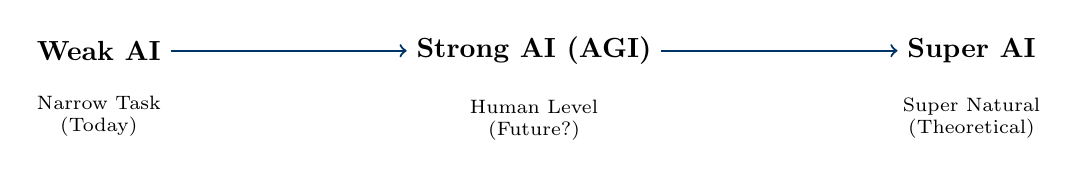
\begin{tikzpicture}
        \node[font=\bfseries] (weak) {Weak AI};
        \node[right=3cm of weak, font=\bfseries] (strong) {Strong AI (AGI)};
        \node[right=3cm of strong, font=\bfseries] (super) {Super AI};
        
        \node[below=0.2cm of weak, align=center, font=\scriptsize] {Narrow Task\\(Today)};
        \node[below=0.2cm of strong, align=center, font=\scriptsize] {Human Level\\(Future?)};
        \node[below=0.2cm of super, align=center, font=\scriptsize] {Super Natural\\(Theoretical)};
        
        \draw[->, thick, ukhblue] (weak) -- (strong);
        \draw[->, thick, ukhblue] (strong) -- (super);
    \end{tikzpicture}
\end{frame}

\begin{frame}{1. Weak AI (Narrow AI)}
    \begin{info_box}{Definition}
        Designed and trained to perform \textbf{one specific task}. It operates within a limited range and lacks consciousness.
    \end{info_box}
    
    \textbf{Examples (All Current AI):}
    \begin{itemize}
        \item \textbf{Virtual Assistants}: Siri, Alexa.
        \item \textbf{Recommenders}: Netflix, Spotify.
        \item \textbf{Self-Driving Cars}: Great at driving, but can't play Chess.
        \item \textbf{ChatGPT}: Great at text, but doesn't "know" what it's saying.
    \end{itemize}
    \vspace{0.5em}
    \textbf{Status:} \textcolor{forestgreen}{\textbf{Exists Today.}}
\end{frame}

\begin{frame}{2. Strong AI (General AI / AGI)}
    \begin{info_box}{Definition}
        A theoretical form of AI that possesses \textbf{human-level intelligence}. It can understand, learn, and apply knowledge to \textit{any} problem.
    \end{info_box}
    
    \begin{itemize}
        \item Would have consciousness, empathy, and self-awareness.
        \item Indistinguishable from a human mind.
    \end{itemize}
    

    \vspace{0.5em}
    \textbf{Status:} \textcolor{alertred}{\textbf{Does Not Exist Yet.}}
\end{frame}

\begin{frame}{3. Super AI (Superintelligence)}
    \begin{info_box}{Definition}
        A theoretical form of AI that \textbf{surpasses human intelligence} in every aspect—creativity, problem-solving, and social skills.
    \end{info_box}
    
    \textbf{Potential Capabilities:}
    \begin{itemize}
        \item Solving global crises (Climate Change, Poverty).
        \item Eradicating diseases.
        \item Unlocking secrets of the universe.
    \end{itemize}
    \vspace{0.5em}
    \textbf{Status:} \textcolor{alertred}{\textbf{Theoretical Future.}}
\end{frame}

% ============================================================================
% FOUNDATIONS OF AI (3 Slides)
% ============================================================================

\section{Foundations of AI}

% 3. Foundations: The Fuel (Data)
\begin{frame}{Foundations of AI: Data Sets}
    Data is the fuel for AI. The lifecycle of data includes:
    \vspace{1em}
    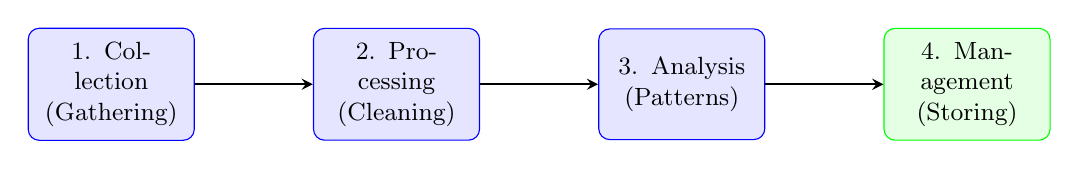
\begin{tikzpicture}[node distance=1.5cm, auto, >=stealth, every node/.style={transform shape}]
        \node[block, fill=blue!10, draw=blue, rounded corners, inner sep=5pt, font=\small, align=center] (coll) {1. Collection\\(Gathering)};
        \node[block, fill=blue!10, draw=blue, rounded corners, inner sep=5pt, font=\small, align=center, right=of coll] (proc) {2. Processing\\(Cleaning)};
        \node[block, fill=blue!10, draw=blue, rounded corners, inner sep=5pt, font=\small, align=center, right=of proc] (ana) {3. Analysis\\(Patterns)};
        \node[block, fill=green!10, draw=green, rounded corners, inner sep=5pt, font=\small, align=center, right=of ana] (mgmt) {4. Management\\(Storing)};
        
        \draw[->, thick] (coll) -- (proc);
        \draw[->, thick] (proc) -- (ana);
        \draw[->, thick] (ana) -- (mgmt);
    \end{tikzpicture}
    \vspace{1em}
    \begin{example_box}{Business Context}
    Collecting customer feedback $\to$ Cleaning it $\to$ Finding trends $\to$ Storing for future strategy.
    \end{example_box}
\end{frame}

% 4. Foundations: The Math
\begin{frame}{Foundations of AI: Mathematics}
    AI is built on a strong mathematical foundation.
    \vspace{1em}
    \begin{columns}
        \column{0.5\textwidth}
        \begin{concept_box}{Key Mathematical Fields}
        \begin{itemize}
            \item \textbf{Statistics}: Handling uncertainty and data trends.
            \item \textbf{Probability}: Predicting likelihood of events.
            \item \textbf{Calculus}: Optimization (changing rates).
            \item \textbf{Linear Algebra}: Handling multi-dimensional data arrays.
        \end{itemize}
        \end{concept_box}
        \column{0.5\textwidth}
        \centering
        \Large $\sum \int \pi$
    \end{columns}
\end{frame}

% 5. Foundations: The Tools (CS)
\begin{frame}{Foundations of AI: Computer Science}
    To implement the math, we need Computer Science tools.
    \vspace{1em}
    \begin{concept_box}{Core CS Concepts}
    \begin{itemize}
        \item \textbf{Programming}: Writing instructions (Python, C++).
        \item \textbf{Data Structures}: Organizing data efficiently (Trees, Graphs).
        \item \textbf{Algorithms}: Step-by-step procedures for calculation.
        \item \textbf{Software Development}: Building robust systems.
    \end{itemize}
    \end{concept_box}
\end{frame}

% ============================================================================
% HISTORY OF AI (4 Slides)
% ============================================================================

\section{History of AI}

\begin{frame}{The Turing Test (1950)}
    \begin{columns}
        \column{0.5\textwidth}
        \textbf{Can machines think?}
        \begin{itemize}
            \item Proposed by \textbf{Alan Turing}.
            \item A test to see if a computer can fool a human into thinking it is also human.
            \item If the human judge cannot tell which is the machine, the machine passes.
        \end{itemize}
        
        \column{0.5\textwidth}
        \centering
        \includegraphics[width=\textwidth,height=0.7\textheight,keepaspectratio]{turing-test.png}
    \end{columns}
\end{frame}

% 6. History Phase 1
\begin{frame}{History of AI: Phase 1 (1950s) - The Birth}
    \textbf{Theoretical Foundation}
    \begin{timeline}
    \begin{itemize}
        \item \textbf{1956: The Name "AI"} \\ At a famous meeting (Dartmouth Conference), scientists officially created the field of "Artificial Intelligence."
    \end{itemize}
    \end{timeline}
\end{frame}

% 7. History Phase 2
\begin{frame}{History of AI: Phase 2 (1960s) - Early Hype}
    \textbf{The First Programs}
    \begin{itemize}
        \item Researchers started building systems that could "talk" and "move."
        \item \textbf{Key Milestones:}
        \begin{itemize}
            \item \textbf{ELIZA}: The first Chatbot.
            \item \textbf{Shakey}: The first Mobile Robot.
        \end{itemize}
    \end{itemize}
\end{frame}

\begin{frame}{ELIZA (1964): The First Chatbot}
    \begin{columns}
        \column{0.45\textwidth}
        \begin{itemize}
            \item Created by \textbf{Joseph Weizenbaum} at MIT.
            \item \textbf{What it did}: Pretended to be a therapist.
            \item \textbf{How it worked}: It looked for keywords. If you said "I feel sad", it simply asked "Why do you feel sad?".
            \item \textbf{Impact}: People thought it was real, even though it didn't understand anything.
        \end{itemize}
        
        \column{0.55\textwidth}
        \centering
        \includegraphics[width=\textwidth,height=0.75\textheight,keepaspectratio]{ELIZA.png}
    \end{columns}
\end{frame}

\begin{frame}{Shakey the Robot (1966)}
    \begin{columns}
        \column{0.5\textwidth}
        \begin{itemize}
            \item Developed at \textbf{SRI International}.
            \item The first \textbf{robot that could move and think}.
            \item \textbf{Capabilities}: It could look at a room and plan how to move across it.
            \item \textbf{Limit}: It was very slow ("shook" while thinking).
            \item \textbf{Legacy}: The "Grandfather" of self-driving cars.
        \end{itemize}
        
        \column{0.5\textwidth}
        \centering
        \includegraphics[width=\textwidth,height=0.75\textheight,keepaspectratio]{shaky.jpg}
    \end{columns}
\end{frame}

% 8. History Phase 3
\begin{frame}{History of AI: Phase 3 (1990s) - Modern Era}
    \textbf{Computers Get Smarter}
    \begin{itemize}
        \item AI started solving specific, complex problems.
        \item \textbf{Key Milestones:}
        \begin{itemize}
            \item \textbf{Deep Blue}: Beating the World Chess Champion.
            \item \textbf{Google Search}: Organizing the world's information.
        \end{itemize}
    \end{itemize}
\end{frame}

\begin{frame}{Deep Blue vs. Kasparov (1997)}
    \begin{columns}
        \column{0.5\textwidth}
        \begin{itemize}
            \item \textbf{The Match}: IBM's Deep Blue played against \textbf{Garry Kasparov} (World Champion).
            \item \textbf{The Result}: Deep Blue won.
            \item \textbf{Significance}: It was the first time a machine defeated a reigning world champion in a complex game.
            \item \textbf{Method}: "Brute Force" search (calculating 200 million positions per second).
        \end{itemize}
        
        \column{0.5\textwidth}
        \centering
        \includegraphics[width=\textwidth,height=0.75\textheight,keepaspectratio]{kasparov.jpg}
    \end{columns}
\end{frame}

% 9. History Phase 4
\begin{frame}{History of AI: Phase 4 (2010s+) - The Revolution}
    \textbf{Deep Learning Takes Over}
    \begin{timeline}
    \begin{itemize}
        \item \textbf{2012: AlexNet}: Computers suddenly got VERY good at recognizing images (Cats vs. Dogs).
        \item \textbf{2022: ChatGPT}: AI learned to write poetry, code, and essays like a human.
    \end{itemize}
    \end{timeline}
\end{frame}

% ...

% 11. The Revolution Answer
\begin{frame}{The Recipe for Revolution}
    It wasn't magic. It was the convergence of three factors:
    \vspace{1em}
    \begin{columns}[t]
        \column{0.31\textwidth}
        \begin{concept_box}{1. Big Data}
            \small Explosion of data from social media and sensors.
        \end{concept_box}
        
        \column{0.31\textwidth}
        \begin{info_box}{2. Hardware}
            \small Faster Computers (GPUs). Gaming tech powering AI.
        \end{info_box}
        
        \column{0.31\textwidth}
        \begin{example_box}{3. Algorithms}
            \small Smarter Math. Better ways to train Deep Networks.
        \end{example_box}
    \end{columns}
\end{frame}

% ============================================================================
% NEW RECOMMENDED SLIDES
% ============================================================================

\begin{frame}{AI Ethics: Why it Matters}
    \begin{quote_box}
        "With great power comes great responsibility."
    \end{quote_box}
    
    As future managers, you must understand the risks:
    \begin{itemize}
        \item \textbf{Bias}: If we train AI on bad data, it makes unfair decisions (e.g., rejecting loans for minorities).
        \item \textbf{Privacy}: Who owns the data? (Your face, your clicks).
        \item \textbf{Deepfakes}: AI generated fake videos/audio. How do we trust what we see?
    \end{itemize}
\end{frame}


\begin{frame}{AI will replace all humans.}
    \begin{tikzpicture}[remember picture, overlay]
        \node[at=(current page.center), yshift=-1cm] {
            \includegraphics[width=\paperwidth, height=0.9\paperheight, keepaspectratio]{aiReplaceHumans.png}
        };
    \end{tikzpicture}
\end{frame}

\begin{frame}{Myths vs. Reality}
    \begin{columns}
        \column{0.5\textwidth}
        \begin{concept_box}{MYTH}
            "AI will replace all humans."
        \end{concept_box}
        
        \column{0.5\textwidth}
        \begin{example_box}{REALITY}
            "AI will replace humans who \textbf{don't} use AI."
        \end{example_box}
    \end{columns}
    
    \vspace{1em}
    \textbf{The Goal:} AI is a \textit{tool} (like Excel or specific software), not a replacement for human creativity and empathy.
\end{frame}

% ============================================================================
% AI DISCIPLINES (6 Slides)
% ============================================================================

\section{AI Disciplines}

% 12. Machine Learning
\begin{frame}{1. Machine Learning (ML)}
    \begin{info_box}{Definition}
        Focuses on developing algorithms that enable computers to \textbf{learn from} and \textbf{make predictions} based on data.
    \end{info_box}
    \begin{example_box}{Business Example}
        \textbf{Prediction}: Predicting numbers (Predicting house prices based on size).
    \end{example_box}
\end{frame}

% 13. NLP
\begin{frame}{2. Natural Language Processing (NLP)}
    \begin{info_box}{Definition}
        Involves the interaction between computers and human language.
    \end{info_box}
    \begin{itemize}
        \item \textbf{Speech Recognition}: Siri, Alexa.
        \item \textbf{Language Translation}: Google Translate (Kurdish $\leftrightarrow$ English).
        \item \textbf{Sentiment Analysis}: Understanding customer emotions in reviews.
        \item \textbf{Text Generation}: Creating essays, code, or emails (ChatGPT).
    \end{itemize}
\end{frame}

\begin{frame}{NLP }
    \begin{columns}
        \column{0.5\textwidth}
        \centering
        \includegraphics[width=\textwidth,height=0.8\textheight,keepaspectratio]{NLP1.png}
        
        \column{0.5\textwidth}
        \centering
        \includegraphics[width=\textwidth,height=0.8\textheight,keepaspectratio]{NLP2.png}
    \end{columns}
\end{frame}

% 14. Computer Vision
\begin{frame}{3. Computer Vision}
    \begin{info_box}{Definition}
        Deals with how computers gain high-level understanding from digital images or videos.
    \end{info_box}
    \begin{itemize}
        \item \textbf{Object Recognition}: Identifying products on a shelf.
        \item \textbf{Image Classification}: Sorting photos (Cat vs Dog).
        \item \textbf{Business Use}: Quality control in factories (spotting defects).
        \item \textbf{Generation}: Creating new images or videos (Midjourney, Sora).
    \end{itemize}
\end{frame}

\begin{frame}{Computer Vision }
    \centering
    \includegraphics[width=\textwidth,height=0.85\textheight,keepaspectratio]{computer vision.png}
\end{frame}

% 15. Robotics
\begin{frame}{4. Robotics}
    \begin{info_box}{Definition}
        Combines AI with mechanical engineering to create robots that perform tasks.
    \end{info_box}
    \begin{itemize}
        \item \textbf{Autonomous}: Robots that work without human help.
        \item \textbf{Assistive}: Robots that help humans lift heavy objects.
    \end{itemize}
\end{frame}

% 16. Expert Systems
\begin{frame}{5. Expert Systems}
    \begin{info_box}{Definition}
        Systems that emulate the decision-making ability of a human expert.
    \end{info_box}
    \begin{itemize}
        \item Uses a knowledge base of rules ("If X then Y").
        \item \textbf{Example}: Medical diagnosis systems or Loan Approval systems in banking.
    \end{itemize}
\end{frame}

% 17. Neural Networks
\begin{frame}{6. Neural Networks \& Deep Learning}
    \begin{info_box}{Definition}
        Algorithms inspired by the structure of the human brain.
    \end{info_box}
    \begin{itemize}
        \item Particularly effective for complex tasks like image and speech recognition.
        \item "Deep Learning" implies many layers of these neural networks.
    \end{itemize}
\end{frame}

\begin{frame}{Neural Network Visualization}
    \begin{columns}
        \column{0.5\textwidth}
        \centering
        \textbf{Bio-Inspiration}
        \includegraphics[width=\textwidth,height=0.75\textheight,keepaspectratio]{neuron_vs_artificial.png}
        
        \column{0.5\textwidth}
        \centering
        \textbf{Architecture}
        \includegraphics[width=\textwidth,height=0.75\textheight,keepaspectratio]{brain_vs_network.png}
    \end{columns}
\end{frame}



% ...

% ============================================================================
% SECTION: ML TYPES (SPLIT)
% ============================================================================

\begin{frame}{Type 1: Supervised Learning}
    \begin{info_box}{"Learning with a Teacher"}
        The computer learns from \textbf{labeled data}. We give it the question and the answer key.
    \end{info_box}
    
    \begin{columns}
        \column{0.6\textwidth}
        \textbf{How it works:}
        \begin{enumerate}
            \item Input: Image of an apple.
            \item Label: "This is an apple."
            \item The model learns to link the image to the name.
        \end{enumerate}
        
        \column{0.4\textwidth}
        \begin{example_box}{Examples}
        \begin{itemize}
            \item Spam classification (Spam/Not Spam)
            \item Face Recognition
            \item Medical Diagnosis
        \end{itemize}
        \end{example_box}
    \end{columns}
\end{frame}

\begin{frame}{Example: Spam Email Filtering}
    \begin{columns}
        \column{0.5\textwidth}
        \begin{concept_box}{Traditional Approach}
            \textbf{Problem:} Manually defining rules.
            \begin{itemize}
                \item "If email contains 'Free Money', delete it."
                \item \textbf{Failure:} Spammers change "Free Money" to "Fr33 M0ney" and the rule fails.
            \end{itemize}
        \end{concept_box}
        
        \column{0.5\textwidth}
        \begin{info_box}{AI Approach (Supervised)}
            \textbf{Solution:} Learning from data.
            \begin{itemize}
                \item Show AI 1,000,000 spam emails and 1,000,000 normal emails.
                \item AI finds the patterns itself (words, sender, time).
                \item Adapts automatically to new tricks.
            \end{itemize}
        \end{info_box}
    \end{columns}
\end{frame}

\begin{frame}[plain]
    \begin{tikzpicture}[remember picture, overlay]
        \node[at=(current page.center)] {
            \includegraphics[width=\paperwidth, height=\paperheight, keepaspectratio]{2.jpg}
        };
    \end{tikzpicture}
\end{frame}

\begin{frame}{Type 2: Unsupervised Learning}
    \begin{info_box}{"Learning without a Teacher"}
        The computer learns from \textbf{unlabeled data}. It must find hidden patterns or structures on its own.
    \end{info_box}
    
    \begin{columns}
        \column{0.6\textwidth}
        \textbf{How it works:}
        \begin{enumerate}
            \item Input: A database of customer purchases.
            \item No labels.
            \item The model groups similar customers together.
        \end{enumerate}
        
        \column{0.4\textwidth}
        \begin{example_box}{Examples}
        \begin{itemize}
            \item Customer segmentation (Marketing)
            \item Product recommendations
            \item Anomaly detection (Fraud)
        \end{itemize}
        \end{example_box}
    \end{columns}
\end{frame}

\begin{frame}[plain]
    \begin{tikzpicture}[remember picture, overlay]
        \node[at=(current page.center)] {
            \includegraphics[width=\paperwidth, height=\paperheight, keepaspectratio]{1.png}
        };
    \end{tikzpicture}
\end{frame}

\begin{frame}{Type 3: Reinforcement Learning}
    \begin{info_box}{"Learning by Trial \& Error"}
        The computer learns by interacting with an environment and receiving \textbf{rewards} or \textbf{punishments}.
    \end{info_box}
    
    \begin{columns}
        \column{0.6\textwidth}
        \textbf{How it works:}
        \begin{enumerate}
            \item Agent takes an action (e.g., moves chess piece).
            \item Environment gives specific feedback (Win = +10, Lose = -10).
            \item Agent optimizes to get max reward.
        \end{enumerate}
        
        \column{0.4\textwidth}
        \begin{example_box}{Examples}
        \begin{itemize}
            \item Playing Chess/AlphaGo
            \item Training Robots to walk
            \item Self-driving cars
        \end{itemize}
        \end{example_box}
    \end{columns}
\end{frame}

\begin{frame}{Reinforcement Learning Example}
    \centering
    \includegraphics[width=\textwidth,height=0.85\textheight,keepaspectratio]{RL.png}
\end{frame}

% ============================================================================
% APPLICATIONS (Engineering Focus) (7 Slides)
% ============================================================================

\section{AI Applications}

% 19. Overview
\begin{frame}{Engineering Applications Overview}
    AI transforms every engineering discipline:
    \begin{itemize}
        \item Mechanical
        \item Electrical
        \item Civil
        \item Chemical
        \item Architecture
        \item Aerospace
    \end{itemize}
\end{frame}





% ============================================================================
% DEEP DIVE: MISCONCEPTIONS & REALITY
% ============================================================================

\section{Misconceptions vs. Reality \\ \vspace{0.3em} \normalfont\footnotesize{(Discussion)}}

\begin{frame}{Misconception 1: AI Understands Meaning}
    \begin{concept_box}{The Myth}
        "AI understands words, images, and concepts just like a human does."
    \end{concept_box}
    
    \begin{example_box}{The Reality}
        \begin{itemize}
            \item AI \textbf{does not} truly understand meaning.
            \item It recognizes \textbf{patterns} and statistical relationships in data.
            \item It lacks consciousness, awareness, or comprehension.
        \end{itemize}
    \end{example_box}
    
    \textbf{Example:} Chatbots (like GPT) generate coherent text based on probability, not because they "know" what they are saying.
\end{frame}

\begin{frame}{Misconception 2: AI Has Emotions}
    \begin{concept_box}{The Myth}
        "AI can feel happy, sad, or empathetic."
    \end{concept_box}
    
    \begin{example_box}{The Reality}
        \begin{itemize}
            \item AI \textbf{does not} have feelings or consciousness.
            \item Emotional responses ("I'm sorry to hear that") are purely \textbf{programmed simulations}.
        \end{itemize}
    \end{example_box}
    
    \textbf{Key Point:} A robot programmed to smile is executing code, not experiencing happiness.
\end{frame}

\begin{frame}{Misconception 3: AI Can Do Everything}
    \begin{concept_box}{The Myth}
        "If a machine is smart, it can solve any problem."
    \end{concept_box}
    
    \begin{example_box}{The Reality: Narrow AI}
        \begin{itemize}
            \item Most AI today is \textbf{Narrow AI}—designed for \textbf{one specific task}.
            \item Knowledge generally does not transfer without retraining.
        \end{itemize}
    \end{example_box}
    
    \textbf{Example:} A Chess champion AI cannot drive a car. A Face Recognition system cannot compose music.
\end{frame}

\begin{frame}{Assumptions Behind AI Research}
    AI isn't magic; it's math.
    
    \begin{concept_box}{The Core Assumption}
        \textbf{"Intelligence can be represented mathematically."}
    \end{concept_box}
    
    \vspace{1em}
    \begin{itemize}
        \item \textbf{Meaning}: Reasoning, learning, and decision-making can be expressed as algorithms and models.
        \item \textbf{Why it matters}: We need to translate "intelligence" into code that a computer can execute.
        \item If we couldn't model it mathematically, we couldn't build AI.
    \end{itemize}
\end{frame}

\begin{frame}{Why These Misconceptions Matter}
    \begin{enumerate}
        \item \textbf{Expectations vs. Reality}: Students shouldn't overestimate what AI can do (leads to disappointment).
        \item \textbf{Ethical Decisions}: Misunderstanding AI leads to misplaced trust (e.g., trusting AI for moral judgment).
        \item \textbf{Design Perspective}: Understanding limitations helps us design better systems.
    \end{enumerate}
    
    \vspace{1em}
    \begin{quote_box}
        \textbf{Analogy}: Think of AI like a \textbf{car}. It's great at transport, but it can't cook dinner. It's a tool with a specific purpose.
    \end{quote_box}
\end{frame}


\begin{frame}
  \centering
  \Huge \textbf{Thank You!}\\
 
  \textbf{Questions?}
\end{frame}

\end{document}
